\documentclass[twocolumn, chapterprefix, headings=big, numbers=enddot, ngerman]{scrreprt}
\usepackage[T1]{fontenc}
\usepackage[ngerman]{babel}
\usepackage[margin=1in]{geometry} %width = 6cm
\usepackage{xcolor}
\usepackage{lipsum}
\usepackage[]{graphicx}
\usepackage{float}
\usepackage[]{hyperref}  % hidelinks
% \graphicspath{ {./pictures/} }
% \newcommand\kw[1]{\textcolor{blue}{\itshape #1}}
% \newcommand\kw[1]{\textbf{\itshape #1}}

\begin{document}
\author{me \and me \and Gustav}
\title{Some things I did}
\date{1st April 2020}
\maketitle
\tableofcontents

% \lipsum[1-2]{}

üäö

Some text\footnote{that's not true} with \emph{emphasis and \emph{nested} content}.
Some text~\ref{subsec:labelone} in \textit{italic and \textit{nested} content}.

\begin{figure}[H]
  \centering
  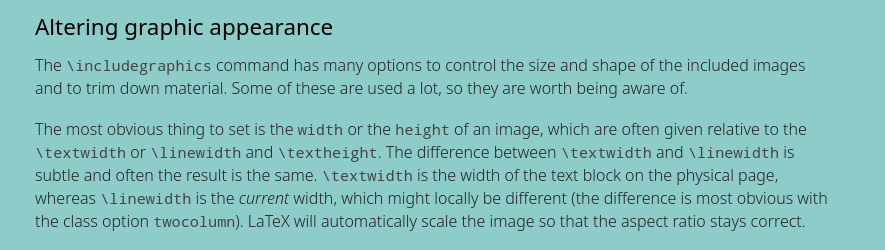
\includegraphics[width=1\textwidth]{./imgs/img.png}
  \caption{An example image}
\end{figure}

\chapter{Aller Anfang ist schwer}

\section{boring}
\subsection{subsection}
\label{subsec:labelone}
\subsubsection{subsubsection}

\begin{figure}[ht]
  \centering
  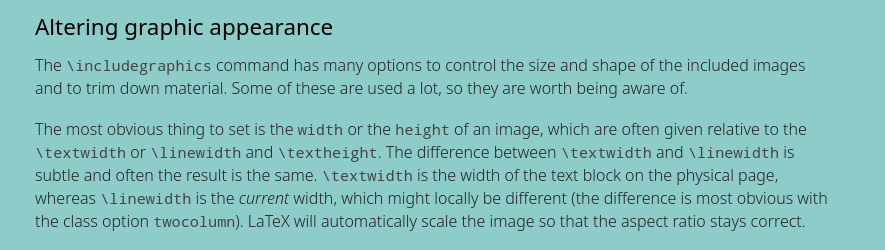
\includegraphics[width=0.8\linewidth]{./imgs/img.png}
  \caption{Name}%
  \label{fig:name}
\end{figure}

\begin{center}
  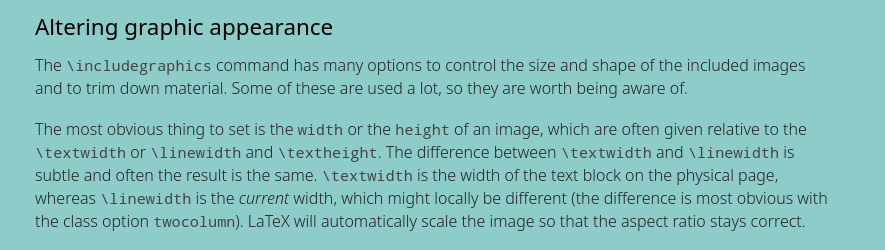
\includegraphics[width=0.95\linewidth]{./imgs/img.png}
\end{center}
\begin{center}
  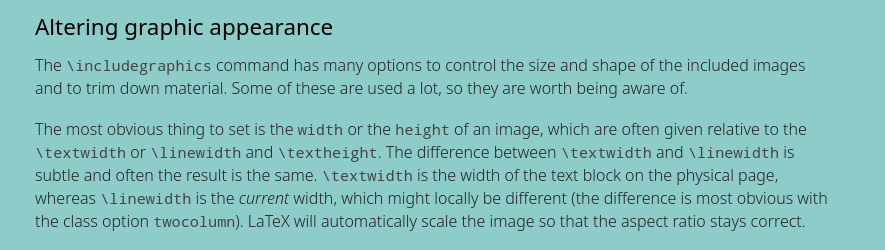
\includegraphics[height=0.05\textheight]{./imgs/img.png}
\end{center}

\paragraph{test}

\[
\frac{12}{3 \cdot 12 + var_3}\frac{asdf}{asdf_{12}}
\]

How is this supposed to work?

How does this work?

Ordered
\begin{enumerate}
  \item An \textcolor{blue}{another one}
  \item Another One
  \item Wow! Three entries
\end{enumerate}

\subparagraph{that's dump}
That makes no sense!

Unordered
\begin{itemize}
  \item An entry
  \item Another One
  \item Wow! Three entries
  \begin{enumerate}
    \item An entry
    \item Another One
    \item Wow! Three entries
  \end{enumerate}
\end{itemize}

\begin{description}
\item[Dog:] member of the genus Canis, which forms part of the wolf-like canids,
  and is the most widely abundant terrestrial carnivore.
\item[Cat:] domestic species of small carnivorous mammal. It is the only
  domesticated species in the family Felidae and is often referred to as the
  domestic cat to distinguish it from the wild members of the family.
\end{description}

Text of material for the first subsection.
\begin{equation}
  e^{i\pi}+1 = 0
\label{eq:labeltwo}
\end{equation}

In subsection~\ref{subsec:labelone} is equation~\ref{eq:labeltwo}.
\end{document}
